\documentclass[margin=10pt]{standalone}
\usepackage{cmbright}
%\renewcommand{\familydefault}{\sfdefault}
%
\usepackage{tikz}
\usetikzlibrary{arrows}
\usetikzlibrary{arrows.meta}
\usetikzlibrary{backgrounds}
\usetikzlibrary{decorations.markings}
\usetikzlibrary{fit}
\usetikzlibrary{matrix}
\usetikzlibrary{positioning}
\usetikzlibrary{shadows}

\begin{document}
{
\normalsize
%\large

\newsavebox\mybox
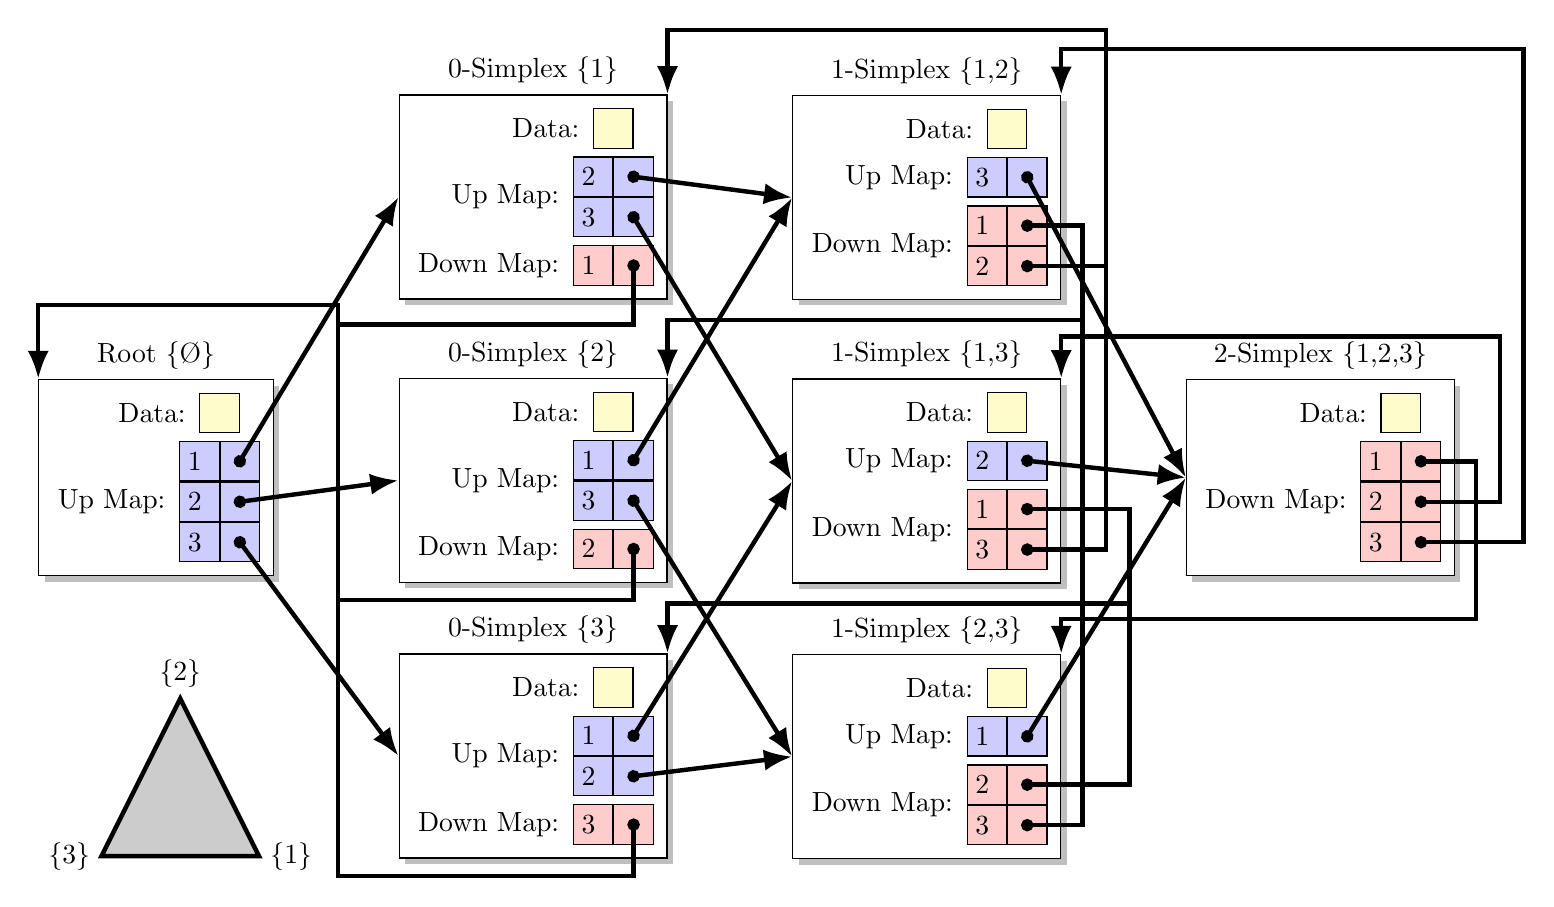
\begin{tikzpicture}[
		every node/.style = {
			draw,
			%text height = 1.5ex,
			fill = white!5,
			align = center,
		},
		labeltxt/.style = {
			draw = none,
			fill = none,
		},
		simplex/.style = {
			drop shadow,
		},
		genmatrix/.style={
			matrix of nodes,
			nodes = {anchor=center},
			nodes in empty cells,
			draw = none,				% remove lines around matrix
			outer sep = 0.5mm,			% allow them to stack better
			inner sep = 0,
			minimum size = 0.5cm,
		},
		upnode/.style = {
			genmatrix,
			nodes = {fill=blue!20},
		},
		downnode/.style = {
			genmatrix,
			nodes = {fill=red!20},
		},
		datanode/.style = {
			genmatrix,
			nodes = {fill=yellow!20},
			label = west:{Data:},
		},
		line/.style = {
			ultra thick,
		},
        ptr/.style = {
			postaction = {decorate,
				decoration={markings,
		            mark=at position 0.0
		                with {
		                    \filldraw[fill=black] circle[radius=0.5mm];
		                }
		        },
		    },
        },
        arr/.style = {
        	-Latex,
        },
 		]

	%\draw[step=1cm,black!80,very thin] (0,0) grid (16,12);
	%\draw[step=0.5cm,black!20,very thin] (0,0) grid (16,12);
	%%%%%%%%%%%%%%%%%%%%%%%%%%%%%
	% Simplex (Root)            %
	% %%%%%%%%%%%%%%%%%%%%%%%%%%%
 	\matrix[upnode,
 			label={[name=rootup-l]west:{Up Map:}}
 		   ]
 		(rootup) at (0,5)
	{
		1 & \\
		2 & \\
		3 & \\
	};
	\matrix[datanode,
			above=0mm of rootup
		   ]
		(rootdata)
	{
		\\
	};

	\begin{scope}[on background layer]
		\node[simplex,
			  label={[name=root-l]north:{Root \{\O\}}},
			  fit=(rootdata)(rootup)(rootup-l)
			 ] (root){};
	\end{scope}

	%%%%%%%%%%%%%%%%%%%%%%%%%%%%%
	% Simplex (1)               %
	% %%%%%%%%%%%%%%%%%%%%%%%%%%%
	\matrix[downnode,
			label={[name=1down-l]west:{Down Map:}}
		   ]
		(1down) at (5,8)
	{
		1 & \\
	};

	\matrix[upnode,
			label={[name=1up-l]west:{Up Map:}},
			above=0mm of 1down
		   ]
		(1up)
	{
		2 & \\
		3 & \\
	};

	\matrix[datanode,
		    above=0mm of 1up
		   ]
		(1data)
	{
		\\
	};

	\begin{scope}[on background layer]
		\node[simplex,
		      label={[name=1-l]north:{$0$-Simplex \{1\}}},
		      fit=(1data)(1up)(1up-l)(1down)(1down-l)
		     ]
		    (1){};
	\end{scope}

	%%%%%%%%%%%%%%%%%%%%%%%%%%%%%
	% Simplex (2)               %
	% %%%%%%%%%%%%%%%%%%%%%%%%%%%
	\matrix[downnode,
			label={[name=2down-l]west:{Down Map:}}
		   ]
		(2down) at (5,4.4)
	{
		2 & \\
	};

	\matrix[upnode,
			label={[name=2up-l]west:{Up Map:}},
			above=0mm of 2down
		   ]
		(2up)
	{
		1 & \\
		3 & \\
	};

	\matrix[datanode,
		    above=0mm of 2up
		   ]
		(2data)
	{
		\\
	};

	\begin{scope}[on background layer]
		\node[simplex,
		      label={[name=2-l]north:{$0$-Simplex \{2\}}},
		      fit=(2data)(2up)(2up-l)(2down)(2down-l)
		     ]
		    (2){};
	\end{scope}

	%%%%%%%%%%%%%%%%%%%%%%%%%%%%%
	% Simplex (3)               %
	% %%%%%%%%%%%%%%%%%%%%%%%%%%%
	\matrix[downnode,
			label={[name=3down-l]west:{Down Map:}}
		   ]
		(3down) at (5,0.9)
	{
		3 & \\
	};

	\matrix[upnode,
			label={[name=3up-l]west:{Up Map:}},
			above=0mm of 3down
		   ]
		(3up)
	{
		1 & \\
		2 & \\
	};

	\matrix[datanode,
		    above=0mm of 3up
		   ]
		(3data)
	{
		\\
	};

	\begin{scope}[on background layer]
		\node[simplex,
		      label={[name=3-l]north:{$0$-Simplex \{3\}}},
		      fit=(3data)(3up)(3up-l)(3down)(3down-l)
		     ]
		    (3){};
	\end{scope}

	%%%%%%%%%%%%%%%%%%%%%%%%%%%%%
	% Simplex {1,2}             %
	% %%%%%%%%%%%%%%%%%%%%%%%%%%%
	\matrix[downnode,
			label={[name=12down-l]west:{Down Map:}}
		   ]
		(12down) at (10,8.25)
	{
		1 & \\
		2 & \\
	};

	\matrix[upnode,
			label={[name=12up-l]west:{Up Map:}},
			above=0mm of 12down
		   ]
		(12up)
	{
		3 & \\
	};

	\matrix[datanode,
		    above=0mm of 12up
		   ]
		(12data)
	{
		\\
	};

	\begin{scope}[on background layer]
		\node[simplex,
		      label={[name=12-l]north:{$1$-Simplex \{1,2\}}},
		      fit=(12data)(12up)(12up-l)(12down)(12down-l)
		     ]
		    (12){};
	\end{scope}

	%%%%%%%%%%%%%%%%%%%%%%%%%%%%%
	% Simplex {1,3}             %
	% %%%%%%%%%%%%%%%%%%%%%%%%%%%
	\matrix[downnode,
			label={[name=13down-l]west:{Down Map:}}
		   ]
		(13down) at (10,4.65)
	{
		1 & \\
		3 & \\
	};

	\matrix[upnode,
			label={[name=13up-l]west:{Up Map:}},
			above=0mm of 13down
		   ]
		(13up)
	{
		2 & \\
	};

	\matrix[datanode,
		    above=0mm of 13up
		   ]
		(13data)
	{
		\\
	};

	\begin{scope}[on background layer]
		\node[simplex,
		      label={[name=13-l]north:{$1$-Simplex \{1,3\}}},
		      fit=(13data)(13up)(13up-l)(13down)(13down-l)
		     ]
		    (13){};
	\end{scope}

	%%%%%%%%%%%%%%%%%%%%%%%%%%%%%
	% Simplex {2,3}             %
	% %%%%%%%%%%%%%%%%%%%%%%%%%%%
	\matrix[downnode,
			label={[name=23down-l]west:{Down Map:}}
		   ]
		(23down) at (10,1.15)
	{
		2 & \\
		3 & \\
	};

	\matrix[upnode,
			label={[name=23up-l]west:{Up Map:}},
			above=0mm of 23down
		   ]
		(23up)
	{
		1 & \\
	};

	\matrix[datanode,
		    above=0mm of 23up
		   ]
		(23data)
	{
		\\
	};

	\begin{scope}[on background layer]
		\node[simplex,
		      label={[name=23-l]north:{$1$-Simplex \{2,3\}}},
		      fit=(23data)(23up)(23up-l)(23down)(23down-l)
		     ]
		    (23){};
	\end{scope}


	%%%%%%%%%%%%%%%%%%%%%%%%%%%%%
	% Simplex {1,2,3}             %
	% %%%%%%%%%%%%%%%%%%%%%%%%%%%
	\matrix[downnode,
			label={[name=123down-l]west:{Down Map:}}
		   ]
		(123down) at (15,5)
	{
		1 & \\
		2 & \\
		3 & \\
	};

	\matrix[datanode,
		    above=0mm of 123down
		   ]
		(123data)
	{
		\\
	};

	\begin{scope}[on background layer]
		\node[simplex,
		      label={[name=123-l]north:{$2$-Simplex \{1,2,3\}}},
		      fit=(123data)(123down)(123down-l)
		     ]
		    (123){};
	\end{scope}

	\pgfmathsetlengthmacro{\base}{0.4cm}
	\pgfmathsetlengthmacro{\offset}{0.3cm}

	% ROOTUP
	% \draw[line,ptr,arr] (rootup-1-2.center) -| ([shift={(\base+\offset,0)}]rootup-1-2.center) |- (1.north west);
	% \draw[line,ptr,arr] (rootup-2-2.center) -| ([shift={(\base+2*\offset,0)}]rootup-2-2.center) |- (2.north west);
	% \draw[line,ptr,arr] (rootup-3-2.center) |- (3.north west);
	\draw[line,ptr,arr] (rootup-1-2.center) -- (1.west);
	\draw[line,ptr,arr] (rootup-2-2.center) -- (2.west);
	\draw[line,ptr,arr] (rootup-3-2.center) -- (3.west);


	% 1UP
	% \draw[line,ptr,arr] (1up-1-2.center) -- ([shift={(\base+\offset,0)}]1up-1-2.center) |- (12.north west);
	% \draw[line,ptr,arr] (1up-2-2.center) -- ([shift={(\base+2*\offset,0)}]1up-2-2.center) |- (13.north west);
	\draw[line,ptr,arr] (1up-1-2.center) -- (12.west);
	\draw[line,ptr,arr] (1up-2-2.center) -- (13.west);
	% 1DOWN
	\draw[line,ptr] (1down-1-2.center) |- (1.5,7.25);

	% 2UP
	% \draw[line,ptr] (2up-1-2.center) -| ([shift={(\base+\offset,0)}]1up-1-2.center);
	% \draw[line,ptr,arr] (2up-2-2.center) -- ([shift={(\base+3*\offset,0)}]2up-2-2.center) |- (23.north west);
	\draw[line,ptr,arr] (2up-1-2.center) -- (12.west);
	\draw[line,ptr,arr] (2up-2-2.center) -- (23.west);
	% 2DOWN
	\draw[line,ptr,arr] (2down-1-2.center) |- (1.5,3.75) |- (1.5,7.5) -| (root.north west);

	% 3UP
	% \draw[line,ptr] (3up-1-2.center) -| ([shift={(\base+2*\offset,0)}]1up-2-2.center);
	% \draw[line,ptr] (3up-2-2.center) -| ([shift={(\base+3*\offset,0)}]2up-2-2.center);
	\draw[line,ptr,arr] (3up-1-2.center) -- (13.west);
	\draw[line,ptr,arr] (3up-2-2.center) -- (23.west);
	% 3DOWN
	\draw[line,ptr] (3down-1-2.center) |- (1.5,0.25) |- (1.5,3.75);

	% 12UP
	% \draw[line,ptr,arr] (12up-1-2.center) -| ([shift={(\base+4*\offset,0)}]12up-1-2.center) |- (123.north west);
	\draw[line,ptr,arr] (12up-1-2.center) -- (123.west);
	% 12DOWN
	\draw[line,ptr,arr] (12down-1-2.center) -| ([shift={(\base+\offset,-1.2)}]12down-1-2.center) -| (2.north east);
	\draw[line,ptr,arr] (12down-2-2.center) -| ([shift={(\base+2*\offset,3)}]12down-2-2.center) -| (1.north east);

	% 13UP
	% \draw[line,ptr] (13up-1-2.center) -| ([shift={(\base+4*\offset,0)}]12up-1-2.center);
	\draw[line,ptr,arr] (13up-1-2.center) -- (123.west);
	% 13DOWN
	\draw[line,ptr,arr] (13down-1-2.center) -| ([shift={(\base+3*\offset,-1.2)}]13down-1-2.center) -| (3.north east);
	\draw[line,ptr] (13down-2-2.center) -| ([shift={(\base+2*\offset,3)}]12down-2-2.center);

	% 23UP
	% \draw[line,ptr] (23up-1-2.center) -| ([shift={(\base+4*\offset,0)}]12up-1-2.center);
	 \draw[line,ptr,arr] (23up-1-2.center) -- (123.west);
	% 23DOWN
	\draw[line,ptr] (23down-1-2.center) -| ([shift={(\base+3*\offset,-1.2)}]13down-1-2.center);
	\draw[line,ptr] (23down-2-2.center) -| ([shift={(\base+\offset,-1.2)}]12down-1-2.center);

	% 123DOWN
	\draw[line,ptr,arr] (123down-1-2.center) -| ([shift={(\base+\offset, -2)}]123down-1-2.center) -| (23.north east);
	\draw[line,ptr,arr] (123down-2-2.center) -| ([shift={(\base+2*\offset, 2.1)}]123down-2-2.center) -| (13.north east);
	\draw[line,ptr,arr] (123down-3-2.center) -| ([shift={(\base+3*\offset, 5.75)}]123down-2-2.center) -| (12.north east);

	\filldraw[line, fill=gray!40] (0.5,0.5) node[labeltxt,right]{\{1\}} -- (-0.5,2.5)node[labeltxt,above]{\{2\}} -- (-1.5,0.5)node[labeltxt,left]{\{3\}} -- cycle;
\end{tikzpicture}
}% end size


\end{document}